\documentclass{amsbook}
\usepackage[utf8]{inputenc}
\usepackage{Ceyhun}
\usepackage{amsTurkish}
\usepackage{caption}

\begin{document}
    \chapter{}
    \hPage{079}
    \theoremstyle{definition}
    \begin{definition}
        Ayrıtları, kapalı bir gezi olarak çizilebilen çizgelere \underline{bağlı Euler çizgesi} denir.
    \end{definition}
    \theoremstyle{definition}
    \begin{definition}
        Her parçası bir Euler çizgesi olan çizgelere \underline{Euler çizgesi} (E) denir.
    \end{definition}
    Şekildeki çizgelerden $Ç_{1}$ Euler çizgesidir. $Ç_{2}$ çizgesi ise Euler çizgesi değildir. Kapalı gezideki düğüm kerteleri çift sayı olduğu için, Euler çizgesinin tanımını
    \begin{figure}[htbp]
      \centering
      \begin{minipage}{0.4\textwidth}
        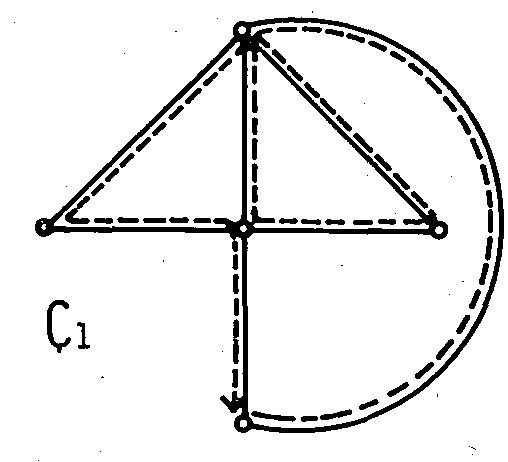
\includegraphics[width=\textwidth]{images/ceyhun-079-fig01.png}
        \caption*{a) Bir Euler çizgesi}
      \end{minipage}
      \begin{minipage}{0.4\textwidth}
        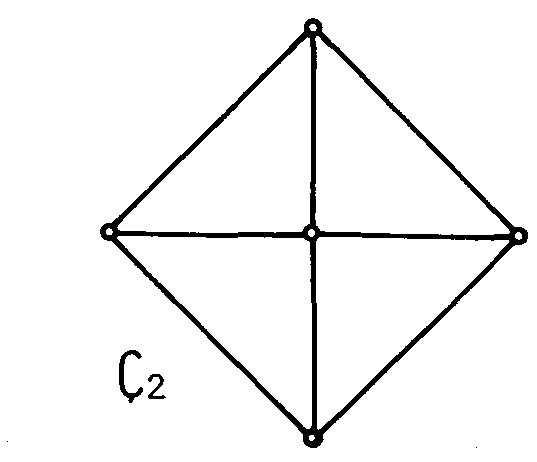
\includegraphics[width=\textwidth]{images/ceyhun-079-fig02.png}
        \caption*{b) Euler olmayan bir çizge}
      \end{minipage}
    \end{figure}
    
    aşağıdaki gibi de verebiliriz.
    \theoremstyle{definition}
    \begin{definition}
        Bütün düğümlerinin kertesi çift sayıya eşit olan çizgelere \underline{Euler çizgesi} denir.
    \end{definition}
    \theoremstyle{definition}
    \begin{definition}
        (Veblen) Ç'nin Euler çizgesi olabilmesi için yeter ve gerek koşul, Ç'nin ortak ayrıtsız çevrelerin birleşiminden oluşmasıdır.
    \end{definition}
\end{document}